\documentclass[enabledeprecatedfontcommands,fontsize=11pt,paper=a4,twoside]{scrartcl}


\newcommand{\grad}{\ensuremath{^{\circ}} }
\renewcommand{\strut}{\vrule width 0pt height5mm depth2mm}

\usepackage[utf8]{inputenc}
\usepackage[T1]{fontenc}
\usepackage[final]{pdfpages}
% obere Seitenränder gestalten können
\usepackage{fancyhdr}
\usepackage{moreverb}
% Graphiken als jpg, png etc. einbinden können
\usepackage{graphicx}
\usepackage{stmaryrd}
% Floats Objekte mit [H] festsetzen
\usepackage{float}
% setzt URL's schön mit \url{http://bla.laber.com/~mypage}
\usepackage{url}
% Externe PDF's einbinden können
\usepackage{pdflscape}
% Verweise innerhalb des Dokuments schick mit " ... auf Seite ... "
% automatisch versehen. Dazu \vref{labelname} benutzen
\usepackage[ngerman]{varioref}
\usepackage[ngerman]{babel}
\usepackage{ngerman}
% Bibliographie
\usepackage{bibgerm}
\usepackage{svg}
% Tabellen
\usepackage{tabularx}
\usepackage{supertabular}
\usepackage[colorlinks=true, pdfstartview=FitV, linkcolor=blue,
            citecolor=blue, urlcolor=blue, hyperfigures=true,
            pdftex=true]{hyperref}
\usepackage{bookmark}



\newcounter{one}
\newcounter{two}[one]
\newcounter{three}[two]

\newcommand{\tone}{0\theone}
\newcommand{\ttwo}{0\thetwo}
\newcommand{\tthree}{0\thetree}
\newcommand{\one}{\stepcounter{one}0\theone}
\newcommand{\two}{\stepcounter{two}0\thetwo}
\newcommand{\three}{\stepcounter{three}0\thethree}
\newcommand\s{\rule{0pt}{4ex}}        
\newcommand{\cb}[1]{{\textcolor{blue}{#1}}}

\usepackage{geometry}
\usepackage{hyperref}
\usepackage{pdfpages} 
\usepackage{colortbl}
%\usepackage{graphicx}   
%\usepackage[utf8x]{inputenc}
\usepackage{fmtcount}
\usepackage[ngerman]{babel}
\usepackage{booktabs}
\usepackage{fancyhdr}
\usepackage[T1]{fontenc}

\usepackage{rotating}

\pagestyle{fancy}
\fancyhf{}

%

%

%

%

\definecolor{dartmouthgreen}{rgb}{0.05, 0.5, 0.06}
\definecolor{color}{rgb}{0.67, 0.88, 0.69}
\definecolor{todo}{rgb}{1.0, 0.41, 0.71}
\definecolor{sort}{rgb}{0.45, 0.76, 0.98}
\definecolor{prob}{rgb}{0.74, 0.83, 0.9}
\definecolor{anw}{rgb}{0.94, 0.86, 0.51}
\usepackage{amsmath}
\usepackage{tabularx}
\usepackage{setspace} 
\hypersetup{
	colorlinks = true,
	linkbordercolor = {white},
	linkcolor=dartmouthgreen,          % color of internal links (change box color with linkbordercolor)
	citecolor=red,        % color of links to bibliography
	filecolor=magenta,      % color of file links
	urlcolor=cyan 
}
\usepackage{geometry}
\geometry{
	a4paper,
	left=20mm,
	right=20mm,
	top=2cm,
	bottom=4cm,
	footskip=4cm
}


\addtolength{\headwidth}{20mm}
\addtolength{\headheight}{2\baselineskip}
\addtolength{\headheight}{0.61pt}


\renewcommand{\headrulewidth}{0pt}
\renewcommand{\headrule}{\vbox to 0pt{\rule{\headwidth}{0.2pt}}}
\setlength{\headsep}{30pt}


\hyphenation{Arbeits-paket}

% Damit Latex nicht zu lange Zeilen produziert:
%\sloppy
%Uneinheitlicher unterer Seitenrand:
%\raggedbottom

% Kein Erstzeileneinzug beim Absatzanfang
% Sieht aber nur gut aus, wenn man zwischen Absätzen viel Platz einbaut
\setlength{\parindent}{0ex}

% Abstand zwischen zwei Absätzen
%\setlength{\parskip}{1ex}

% Seitenränder für Korrekturen verändern
%\addtolength{\evensidemargin}{-1cm}
%\addtolength{\oddsidemargin}{1cm}

%\bibliographystyle{gerapali}

% Lustige Header auf den Seiten
  \pagestyle{fancy}
  \setlength{\headheight}{70.55003pt}
  \fancyhead{}
  \fancyhead[LO,RE]{Software--Projekt 2\\ WiSe 2018/2019
  \\Änderungsdokument}
  \fancyhead[LE,RO]{Seite \thepage\\\slshape \leftmark\\\slshape \rightmark}

%
% Und jetzt geht das Dokument los....
%

\begin{document}

% Lustige Header nur auf dieser Seite
  \thispagestyle{fancy}
  \fancyhead[LO,RE]{ }
  \fancyhead[LE,RO]{Universität Bremen\\FB 3 -- Informatik\\
  Prof. Dr. Rainer Koschke \\Tutor/In: Marcel Steinbeck}
  \fancyfoot[C]{}

% Start Titelseite
  \vspace{3cm}

  \begin{minipage}[H]{\textwidth}
  \begin{center}
  \bf
  \Large
  Software--Projekt 2 WiSe 2018/2019\\
  \smallskip
  \small
  VAK 03-BA-901.02\\
  \vspace{3cm}
  \end{center}
  \end{minipage}
  \begin{minipage}[H]{\textwidth}
  \begin{center}
  \vspace{1cm}
  \bf
  \Large Änderungsdokument \\ 
  \vspace{1cm}
  \Huge\textbf{GraphIt}\normalsize \\
  \vspace{1cm}
  
\includegraphics[width=2.5in]{logo_graphit.png}	
  \vfill
  \end{center}
  \end{minipage}
  \vfill
  \begin{minipage}[H]{\textwidth}
  \begin{center}
  \sf
  \begin{tabular}{lr}
  Anthony Mendil & antmen@tzi.de \\
  Bastian Rexhäuser & brexhaeu@tzi.de\\
  Clement Phung & clement1@tzi.de \\
  Jacky Philipp Mach & machja@tzi.de \\
  Jonah Jaeger & jjaeger@tzi.de \\
  Nina Unterberg & nin\_unt@tzi.de \\
  \end{tabular}
  \\ ~
  \vspace{2cm}
  \\
  \it Abgabe: 10. März 2019\\ ~
  \end{center}
  \end{minipage}

% Ende Titelseite
% Start Leerseite
\thispagestyle{empty}
\cleardoublepage
% Ende Leerseite
\newpage

  \thispagestyle{fancy}
  \fancyhead{}
  \fancyhead[LO,RE]{Software--Projekt \\  2018/2019
  \\Änderungsdokument}
  \fancyhead[LE,RO]{Seite \thepage\\\slshape \leftmark\\~}
  \fancyfoot{}
  \renewcommand{\headrulewidth}{0.4pt}
  
  
  \tableofcontents

\newpage
\section{Einleitung}

Dieses Dokument ist eine Ergänzung zu der Software \textbf{GraphIt}, die im Rahmen des Wintersemesters 2018/19 von der Gruppe \textit{TeamBlank} entwickelt wurde. Inhaltlich beschäftigt sich das Änderungsdokument mit der Beschreibung von Abweichungen zwischen der Architekturbeschreibung und der tatsächlich Implementierung der Anwendung und ergibt dementsprechend auch nur in Kombination mit diesen Abgaben einen Sinn. Es kann also nicht als alleinstehendes Dokument betrachtet werden.  Dies angesprochenen Abweichungen können sich auf Aufbau der Software, auf ihre Bestandteile sowie auf die Zusammenhänge zwischen den Bestandteilen beziehen. In diesem Dokument wird ferner versucht, die Diskrepanzen zu erklären. Als Ausgangspunkt für die folgenden Ausführungen wird dabei die Architekturbeschreibung herangezogen. Durch diesen Ansatz sollen die Abweichungen und deren Erklärungen möglichst nachvollziehbar gemacht werden. Schließlich kommt eine derartige Beschreibung dem praktizierten Vorgehen am nächsten. Denn wir \textit{TeamBlank} als Projektteam sind bei der Umsetzung der Anforderungen an die Software in Quellcode auch von der Architekturbeschreibung ausgegangen und sind nur dann von den in diesem Dokument festgehaltenen Ansätzen abgewichen, wenn es uns als sinnvoll  erschienen ist. Die formale Ausgestaltung dieses Dokuments richtet sich demnach nach dem Projektablauf. \\ 
Dieses Änderungsdokument geht dabei in erster Linie auf die beiden folgenden Abschnitte der Architekturbeschreibung ein: Zum einen werden wir Bezug zu den Problemkarten und den darin erwähnten Strategien nehmen, die im Rahmen der globalen Analyse ausgearbeitet wurden. In diesem Kontext werden wir darlegen, ob die geplanten Strategien zur Lösung der jeweiligen Probleme sich in der praktischen Umsetzung wiederfinden. Ist dies nicht der Fall, wird begründet, warum wir uns für eben diese Abweichung entschieden haben. Zum anderen wird das Datenmodell unseres jetzigen Systems im Abgleich mit dem in der Architekturbeschreibung angedachten Datenmodell beschrieben. Hierzu ist auch ein Diagramm zum neuen Datenmodell vorzufinden, welches grundlegend für die \textbf{GraphIt}-Anwendung in ihrer jetzigen Umsetzung ist. \\
Da sich konzeptionell nichts an der Struktur unser Anwendung geändert hat und auch die fertig implementierten Module der Ausgestaltung IHRER Gegenstücke aus der Modulsicht zu großen Teilen ähneln, hat sich nichts maßgebliches an der Art geändert, wie die Teile unseres System zur Ausführungszeit zusammenwirken. Aus diesen Gründen werden wir nicht weiter auf die konzeptionelle und die Ausführungssicht eingehen. \\
\newpage

\section{Problemkarten}
\emph{Autoren: Bastian Rexhäuser, Jonah Jaeger, Clement Phung, Nina Unterberg}

\subsection{Problemkarte 02 Persistierungsintervall des Graphen}
Die Fragen, in welchen festgelegten Zeitintervall das Syndrom persistiert und abgespeichert werden sollte, wurde in der Architekturbeschreibung mit der Strategie \textbf{S4 - Command} beantwortet. Der Unterschied zu der Architekturbeschreibung und der eigentlichen Umsetzung liegt nun darin, dass der Graphen nicht nach jedem, sondern nur nach ausgewählten Commands persistieren. Zusätzlich haben wir auch den \textbf{Benutzer (S5 – Benutzer)} mit in den Speicherprozess mit eingebunden. Dieser kann den Graphen auch manuell speichern und öffnen. \\

\subsection{Problemkarte 08: Auswertung von Grapheigenschaften}
Für die Auswertung des Graphen bezüglich seiner Eigenschaften wurde in der Architekturbeschreibung angedacht, sowohl \textbf{S22 - JUNG}, \textbf{S24 - eigene Implementierung} und \textbf{S25 - JGraphT} anzuwenden. In der Implementierung haben wir darauf verzichtet \textbf{S22 - JUNG} umzusetzen, da wir durch \textbf{S25} und \textbf{S24} den Funktionsumfang bereits abgedeckt hatten. \\

\subsection{Problemkarte 12: Protokoll der Nutzerinteraktionen exportieren/ importieren}
Um die Anforderungen zu erfüllen, die besagen, dass wir das Protokoll sowohl lesbarer, als auch in maschinell nutzbarer Form exportierbar sein müssen, hatten wir in der Architekturbeschreibung den Export per \texttt{.json}-Datei festgelegt. Wir haben uns nun überlegt, eine für den Nutzer besser lesbare Version exportierbar zu machen. Um eine maschinelle verwendbare Version zu erhalten, muss der Graph als \texttt{.oof} gespeichert werden.\\

\subsection{Problemkarte 13: Benutzeroberfläche}
In der Architekturbeschreibung haben wir festgelegt, dass wir die Benutzeroberfläche mit \textbf{S34 - Framework JavaFX} realisieren. Zusätzlichen haben wir nun in der Implementierung das Framework JFoenix mit eingebunden. JFoenix ist ein Framework, welches auf JavaFX aufbaut. Dies wurde angewendet, um eine hohe Usability unseres Programms anzustreben.\\


\subsection{Problemkarte 25: Persistierung der Parameter in die DB als JSON-String}
In der Architekturbeschreibung haben wir uns entschieden, die Parameter mit \textbf{S63 - Jackson} in JSON-Strings umzuwandeln. Im Laufe der Implementierung sind wir auf \textbf{S54 - GSON} umgestiegen. Hauptsächlicher Grund dafür waren, dass GSON besser in der Handhabung ist. \\


\subsection{Problemkarte 26: Dependency Injection}
Auf Dependency Injection wurde gänzlich in der Implementierung verzichtet und somit wurde auch die angedachte Strategie \textbf{S66 – Google Guice} nicht umgesetzt. Vor allem haben wir drauf verzichtet, da uns die Vorteil gegenüber dem Aufwand nicht ausreichend war. \\


\newpage
\section{Datensicht}
\label{sec:datensicht}

\emph{Autoren: Anthony Mendil, Clement Phung, Bastian Rexhäuser}\\ \\

Im Folgenden beschreiben wir die Datensicht unserer fertig implementierten Anwendung \textit{GraphIt}. Bei der Beschreibung dieser Sicht nehmen wir Bezug zu den folgenden Strategien aus der Architekturbeschreibung: S1 - GXL, S4 - Command, S5 - Benutzer, S7 - Datenmodell, S19 - JUNG, S33 - JavaScript Object Notation (.json), S39 - Eigene Implementierung, S43 - Eigener Datentyp, S45 - H2 Database, S63 - Jackson und S64 - Google Guice. Außerdem werden wir auf die Strategien S50 - Hibernate, S56 - GXL-Framework (bei Source Forge gehostet) und S61 - Regeln in der GXL-Datei eingehen. Im Gegensatz zur Architekturbeschreibung, in der lediglich das geplante Vorgehen beschrieben und auf der Grundlage der eben genannten Strategien begründet wurde, werden wir in diesem Dokument einen Abglich zwischen dem geplanten und dem tatsächlich realisierten Datenmodell machen. \\

Wie in der Architekturbeschreibung erklärt wurde, haben wir nicht geplant, alleine für den Graphen ein komplett eigenes Datenmodell zu erstellen. Stattdessen haben wir geplant das vom Framework JUNG vorgegebene Datenmodell zu verwenden und mit unseren eigenen Datenklassen \texttt{Vertex} (für Knoten) und \texttt{Edge} zu erweitern (für Kanten) (S19 - JUNG). Dieses Vorgehen war zentraler Bestandteil im Rahmen der Implementierung und wurde wie geplant realisiert.\\ 
Die \texttt{Vertex}-Klasse hat (wie geplant) neben den naheliegenden Attributen auch noch weitere Attribute. Je ein Attribut speichert für jeden Relationstyp seinen Eintrittspunkt am Rand des Symptoms in Form eines \texttt{ScopePoint} in einer \texttt{Map}. Ein Element der Aufzählung \texttt{ScopePoint} sollte dabei das Quartal eines Knoten darstellen, in welches eine Pfeilspitze auf ein Knoten andockt. Pfeilspitzen von Kanten, welche in das selbe Quartal führen und den gleichen Pfeilspitzen-Typ haben, sollten in der Visualisierung zusammengefasst dargestellt werden. Das beschriebene Herangehen hat sich nur insofern verändert, als dass nicht nur Quartale erfasst werden, sondern der Rand eines Knoten nun in acht gleich große Teile aufgeteilt wird. Dies ermöglicht es die Kantenbündelung feiner zu justieren. Es ist daneben zu weiteren Änderungen in der \texttt{Vertex}-Klasse gekommen. Sie enthält jetzt weitere (vorher nicht vorgesehene) Attribute. Diese dienen entweder der Speicherung weiterer visueller Eigenschaften (Textgröße, Schriftart) oder sind für die Sperrung einiger Werte dieses Symptoms nötig, um dessen Bearbeitungsmöglichkeiten an die über eine Vorlage spezifizierten Regeln einzuschränken.\\

Wie geplant wurde die Klasse \texttt{Sphere} (zur Realisierung von Sphären) implementiert und mit ihr das vorgegebene Datenmodell erweitert (genauer gesagt erweitert unsere Klasse \texttt{SydromGraph} die Klasse \texttt{DirectedSparseGraph} von JUNG). Auch die Änderungen in dieser Klasse lassen sich auf hinzugekommene Attribute zurückführen. Diese werden aus den selben Gründen benötigt, wie es bei der \texttt{Vertex}-Klasse der Fall ist.
Für die Speicherung des Graphen sowie von allen nötigen Informationen existiert die Klasse \texttt{Syndrom}. Sie fasst den Graphen, die Vorgaben/Bearbeitungsregeln über den ganzen Graph(\texttt{Template}), sowie die zum Rendern und zur Visualisierung benötigten Komponenten von JUNG zusammen. Bei Aspekten diesbezüglich sind wir konzeptionell wie geplant vorgegangen. Lediglich bei den Attributen ist es zu leichten Veränderungen gekommen.\\ 

Die soeben erwähnte \texttt{Template}-Klasse ermöglicht es ein Maximum an Sphären, Knoten (im Graphen insgesamt), Knoten in einer Sphäre und Kanten festzulegen. Des Weiteren können die Arten der erlaubten Kanten eingeschränkt werden, die der Benutzer nicht mehr benutzen darf. Die Funktionalität der Vorlage wurde so umgesetzt, wie wir es angedacht haben. Allerdings haben sich die Attribute verändert, da wir nicht die gesamten Werte, die die Bearbeitungslogik betreffen in der \textit{template}-Klasse speichern. Stattdessen wurden diese Aspekte an die einzelnen Klassen, die Graphelemente beschreiben (\texttt{Sphere}, \texttt{Vertex} und \texttt{Edge}) ausgelagert. \\

Die Klasse \texttt{Values} enthält einige Werte, die beim Erzeugen eines neuen Graph-Objekts (\texttt{Sphere}, \texttt{Vertex} und \texttt{Edge}) benötigt werden. \texttt{Values} ist eine Singleton-Klasse, damit alle Klassen des Systems, die die Werte aus \texttt{Values} benötigen, auf die gleichen Wertebelegungen zugreifen können. Die Nutzerinteraktion in der GUI beeinflussen die Werte, die in \texttt{Values} gesetzt sind. Stellt der Nutzer beispielsweise die Standardfarbe für neue Symptome um, so wird der entsprechende Wert in der Klasse \texttt{Values} angepasst, sodass neu erzeugte Symptome diese Farbe haben. Die Klasse \textit{Values} hat sich gegenüber ihrer geplanten Ausgestaltung insofern geändert, als dass sie weitere Attribute bekommen hat. Diese sind für weitere visuellen Eigenschaften erforderlich, die wir in der Architekturbeschreibung nicht vorgesehen hatten.\\

Um die Persistenz von Daten zu gewährleisten, verwenden wir die eingebettete Datenbank H2 Database in unserem System (S45 - H2). Bei der Kommunikation mit der Datenbank wird das Framework Hibernate genutzt, welches es unter Verwendung von JPA ermöglicht, Objekte (als Instanzen von Klassen) unseres Systems in eine relationale Datenbank zu persistieren (S50 - Hibernate). Hierbei findet ORM (Object-Relational Mapping) Anwendung. Bei der Persistierung von Systemdaten haben wir uns an das vorehen gehalten, das wir im Rahmen der Architekturbeschreibung vorgesehen haben.\\ 

Um den Graphen zu speichern bietet sich die GXL-Repräsentation aus den in der Entscheidung für S1 - GXL genannten Gründen an. Ein als Text-Repräsentation vorliegender Graph wird dabei mit einer Identifikationsnummer versehen und in einer Tabelle unserer Datenbank persistiert. Die Realisierung der genannten Konstruktion lässt sich in der zugehörigen Mapping-Klasse \texttt{Graph} wiederfinden.  An dieser Stelle ist anzumerken, dass wir uns dafür entschieden haben, in der Datenbank immer höchstens einen Graphen zu speichern. Die Tabelle mit den Graphen hat dementsprechend maximal einen Eintrag. Immer wenn versucht wird, einen neuen Graphen zu erstellen oder einen alten zu importieren, wird der Nutzer gefragt, ob er seinen aktuellen Graphen (inklusive festgehaltenem Nutzerverhalten) vorher exportieren möchte, da die Datenbank beim Import (und dem Neuerstellen eines Graphen) geleert wird. Dieses Konzept wurde wie angedacht umgesetzt. Es ist allerdings ebenso möglich lediglich den Graphen ohne Informationen zum Nutzerverhalten zu exportieren.\\
Die Übersetzung unseres Graphen in das GXL-Format erfolgt wie vorher angedacht unter Nutzung des bei Sourceforge gehosteten GXL-Frameworks (S56 - GXL-Framework). Falls der Benutzer eine Vorlage erstellt, werden auch die darin für die Syndrom-Erstellung gesetzten Einschränkungen in selbiger GXL festgehalten (S61 - Regeln in der GXL-Datei). Auch bei diesem Vorgehen halten wir uns an den in den Architekturbeschreibung definierten Plan.\\ 

Die Nutzerinteraktionen mit dem Graphen werden, wie auch der Graph selbst, in der embedded H2 Database gespeichert. Für die Nutzerinteraktionen existiert eine eigene Tabelle in der Datenbank sowie eine zugehörige Mapping-Klasse \texttt{Log}, welche für jeden Eintrag die relevanten Informationen enthält (Strategie S7 - Datenmodell). Zu diesen Informationen gehört auch ein Text im JSON-Format, der aus dem jeweiligen Parameterobjekt erzeugt wird (S33 - JavaScript Object Notation (.json)). Als Bibliothek zum Serialisieren und Deserialisieren der Parameterobjekte in das genannte Format kam bei der Implementierung Gson zum Einsatz. Die in der Architekturbeschreibung vorgesehene Bibliothek war für diesen Fall Jackson(S63 - Jackson). Aber aufgrund mangelnder Erfahrung der Gruppe in diesem Bereich wurde Strategie S64 - Gson umgesetzt, da diese Bibliothek leichter einen Einstieg für Anfänger gewährt.\\
Es sei explizit erwähnt, dass zu einem Log ein Graph gehört, der Graph dennoch nichts vom Log weiß und von diesem auch keine Informationen lesen kann (Many-to-One Beziehung). Auch dieser Ansatz entspricht dem Geplanten. Anders als in der Architekturbeschreibung geplanten Strategie S4 - Command wird nicht nach jeder möglichen Action die Nutzeraktion mit den jeweiligen Parametern und der Graph in dem Zustand persistiert. Dies geschieht nun nur nach bestimmten Actions, welche sich für die Untersuchung der Nutzerinteraktionen des Betrachters als wichtig erscheinen. Obwohl in Strategie S5 - Benutzer festgehalten wurde, dass der Benutzer nicht in der Lage sei, durch einen Speicherbefehls den Graphen zu persistieren, kann der Benutzer dies nun tun. Denn genau genommen kann das Speichern des Graphen in einer externen Datei auch als Persistierung gewertet werden. Die Repräsentation des Graphen in der Datenbank kann jedoch nicht durch ein Befehl des Benutzers gesichert werden.\\
Die bereits erwähnten Parameterklassen sind Unterklassen der Klasse \texttt{Param} - so wie wir es in der Architekturbeschreibung angestrebt haben. Jede dieser Parameter-Klassen gehört speziell zu einer Aktion, für die sie die nötigen Informationen enthält. Hinzufügende und entfernende Aktionen gleicher Art sowie aktivierende und deaktivierende gleicher Art benutzen die gleichen Parameter-Klassen, da die Struktur der Parameterklassen sich stark ähneln würden. Beispielsweise haben demnach die Aktionen des Hinzufügens und Entfernens mehrerer Kanten beide ein \texttt{AddRemoveVerticesParam}. Je nach Aktion werden diese Informationen bei der Ausführung unterschiedlich verwendet. Es ist ebenso anzumerken, dass die einzelnen Parameter-Klassen im Diagramm individuell Assoziationen zu den Klassen \texttt{Vertex}, \texttt{Edge} und \texttt{Sphere} hätten, je nachdem welche Attribute sie besitzen. Um Übersichtlichkeit zu bewahren haben wir im Diagramm nicht alle Parameter-Klassen mit ihren zugehörigen Attributen dargestellt, sondern exemplarisch drei solcher Klassen ausgewählt. Alle Parameter-Klassen lassen sich im Package \texttt{log\_management.parameters} finden. Auch die Verarbeitung dieser Parameterklassen im jetzigen Programm leicht der angedachten Verarbeitungsweise. \\

In unserem Programm ist ebenfalls das Exportieren einzelner Graphen mit den zugehörigen Log-Einträgen möglich. Dies geschieht anhand eines selbst entwickelten Dateiformates (OOF für \glqq out of frameworks\grqq; S43 - eigener Datentyp). Dieses Datei-Format findet für genau diesen Zweck bereits in der Architekturbeschreibung Erwähnung.  \\

%<<<<<<< HEAD
%\newpage
%\label{sec:datensicht}


\textit{Anmerkungen zu dem Diagramm}: \\
Alle dargestellten Attribute sind \texttt{private}. Auch wenn für die Attribute Getter und Setter (außer bei sämtlichen Id's, dort nur Getter) existieren, werden sie aufgrund ihrer Deklaration als \textit{private} im Diagramm markiert. \\
Des weiteren lassen sich die Rollennamen direkt aus den Klassennamen herleiten, weshalb wir sie im Diagramm nicht explizit nennen. Die Assoziation zwischen \texttt{Vertex} und \texttt{ScopePoint} betreffend, wurde beschlossen, dass \texttt{Vertex} statt einem Attribut, in welchem die verschiedenen \texttt{ScopePoints} für die jeweils gleichen Arten der Relationstypen zusammengefasst werden, drei Attribute gegeben werden, die jeweils ausschließlich gleichartige \texttt{ScopePoints} eines Relationstyps beinhalten. Diese Unterteilung sorgt für eine klare logische Trennung und ermöglicht es ohne Filterung direkt auf die \texttt{ScopePoints} zuzugreifen, die einem Pfeiltyp entsprechen. Es muss also nicht erst die Liste aller \texttt{ScopePoints} nach der Art der Relation gefiltert werden.\\


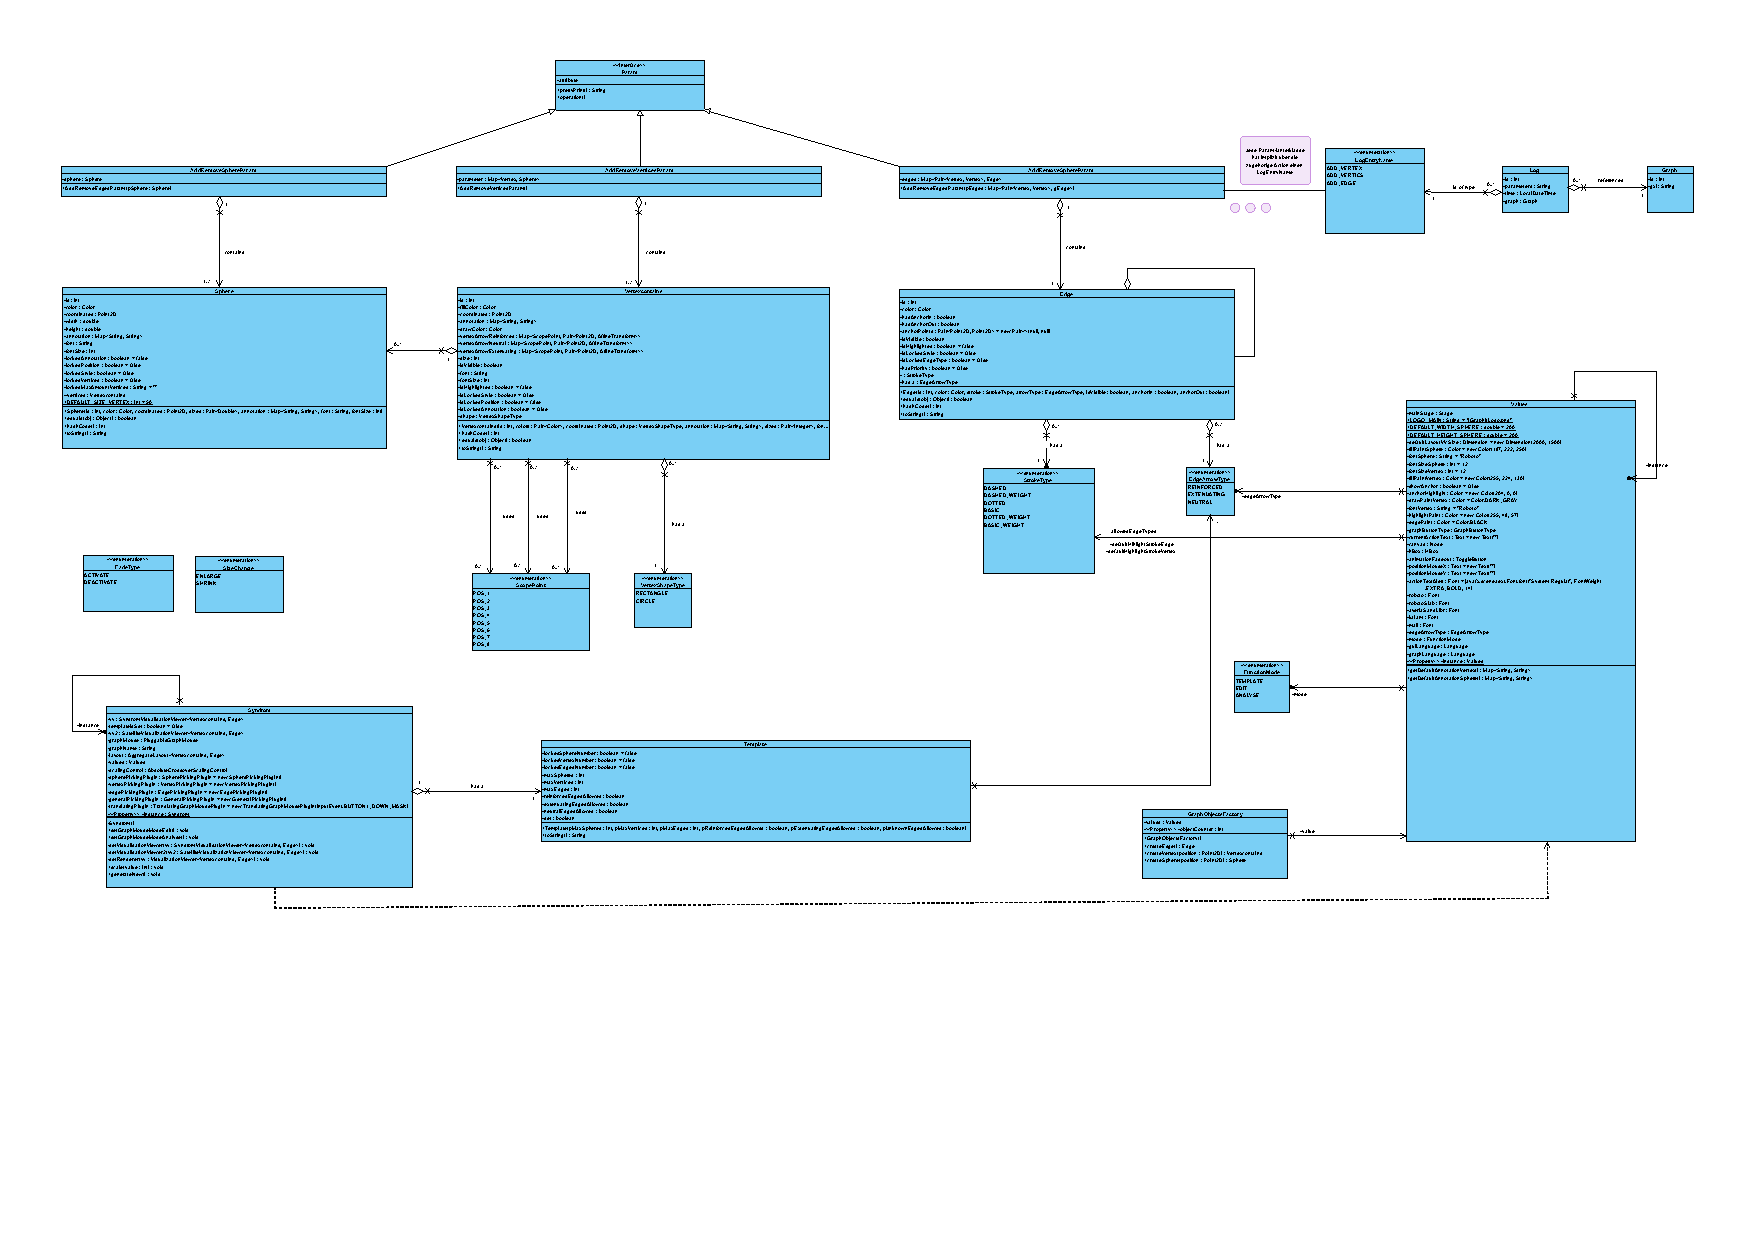
\includepdf[pages=-, landscape, scale=0.77,pagecommand={\null\enlargethispage{2\baselineskip}\vfill\captionof{figure}{Konteptionelle Sicht},\pagestyle{fancy}}]{DatenmodellSVG.pdf}



\end{document}


%%% Local Variables:
%%% mode: latex
%%% mode: reftex
%%% mode: flyspell
%%% ispell-local-dictionary: "de_DE"
%%% TeX-master: t
%%% End:
